\documentclass[11pt]{article}
% ---------------------------------------------------------------
% R3.07 SQL dans un langage de programmation -- preambule commun des sujets de TP
% Article clair, fond blanc, accents de couleur coherents avec les slides
% Charte derivee de R5.A.08 Qualite de developpement (meme palette IUT)
% Utilisation :
%   \documentclass[11pt]{article}
%   % ---------------------------------------------------------------
% R3.07 SQL dans un langage de programmation -- preambule commun des sujets de TP
% Article clair, fond blanc, accents de couleur coherents avec les slides
% Charte derivee de R5.A.08 Qualite de developpement (meme palette IUT)
% Utilisation :
%   \documentclass[11pt]{article}
%   % ---------------------------------------------------------------
% R3.07 SQL dans un langage de programmation -- preambule commun des sujets de TP
% Article clair, fond blanc, accents de couleur coherents avec les slides
% Charte derivee de R5.A.08 Qualite de developpement (meme palette IUT)
% Utilisation :
%   \documentclass[11pt]{article}
%   \input{../../latex/common/r307-tp-preamble.tex}
%   \begin{document}
%   \rtpheader{1}{Titre du TP}
% ---------------------------------------------------------------
\usepackage[T1]{fontenc}
\usepackage[utf8]{inputenc}
\usepackage[french]{babel}
\usepackage[scale=0.92]{tgheros}
\usepackage{tgpagella}
\usepackage[a4paper, margin=2.2cm, headheight=14pt]{geometry}
\usepackage{graphicx}
\usepackage{xcolor}
\usepackage{listings}
\usepackage[skins,listings,breakable]{tcolorbox}
\usepackage{enumitem}
\usepackage{booktabs}
\usepackage{array}
\usepackage{multirow}
\usepackage{tikz}
\usetikzlibrary{shapes, shapes.geometric, arrows, arrows.meta, positioning, calc}
\usepackage[colorlinks=true, linkcolor=qaaccentdark, urlcolor=qaaccentdark]{hyperref}
\usepackage{fancyhdr}
\usepackage{lastpage}
\usepackage{titlesec}
\usepackage{etoolbox}

% ---------------------------------------------------------------
% PALETTE -- version imprimable des couleurs des diapositives
% ---------------------------------------------------------------
\definecolor{qaaccentdark}{HTML}{7A1680}   % violet du logo IUT, fonce pour rester lisible sur blanc
\definecolor{qaaccent2dark}{HTML}{9B4B94}  % violet clair du logo IUT (accent secondaire)
\definecolor{qapanellight}{HTML}{F4F6F8}   % fond de bloc tres clair
\definecolor{qalinelight}{HTML}{D8DEE4}    % filets
\definecolor{qatextdark}{HTML}{1A1D23}     % texte principal
\definecolor{qamuteddark}{HTML}{5B6472}    % texte secondaire
\definecolor{qacodekwl}{HTML}{7A1680}      % code : mots-cles
\definecolor{qacodestrl}{HTML}{2E7D32}     % code : chaines
\definecolor{qacodecoml}{HTML}{6B7280}     % code : commentaires
\definecolor{qacodeannl}{HTML}{B26A00}     % code : annotations / javadoc

\color{qatextdark}

\setlength{\parskip}{4pt}
\setlength{\parindent}{0pt}

% ---------------------------------------------------------------
% TITRES DE SECTION -- texte blanc sur bande de couleur pleine largeur
% (gere aussi les variantes etoilees \section*)
% ---------------------------------------------------------------
\newcommand{\qasectionband}[2]{%
  \noindent\colorbox{#1}{%
    \parbox[c]{\dimexpr\linewidth-2\fboxsep\relax}{%
      \color{white}#2%
    }%
  }%
}
\newcommand{\secformat}[1]{\qasectionband{qaaccentdark}{\bfseries\Large\thesection\quad #1}}
\newcommand{\secformatnn}[1]{\qasectionband{qaaccentdark}{\bfseries\Large #1}}
\newcommand{\subsecformat}[1]{\qasectionband{qaaccent2dark}{\bfseries\large\thesubsection\quad #1}}
\newcommand{\subsecformatnn}[1]{\qasectionband{qaaccent2dark}{\bfseries\large #1}}

\titleformat{\section}{\normalfont}{}{0pt}{\secformat}
\titleformat{name=\section,numberless}{\normalfont}{}{0pt}{\secformatnn}
\titleformat{\subsection}{\normalfont}{}{0pt}{\subsecformat}
\titleformat{name=\subsection,numberless}{\normalfont}{}{0pt}{\subsecformatnn}
\titleformat{\subsubsection}{\normalfont\bfseries\color{qaaccentdark}}{\thesubsubsection}{0.6em}{}
\titlespacing*{\section}{0pt}{14pt}{8pt}
\titlespacing*{\subsection}{0pt}{10pt}{6pt}
\titlespacing*{\subsubsection}{0pt}{8pt}{4pt}

% ---------------------------------------------------------------
% LISTINGS -- theme clair (lstlisting reste utilisable tel quel)
% \lstcode : police + couleur de base, a reutiliser dans les surcharges
% ---------------------------------------------------------------
\newcommand{\lstcode}{\ttfamily\color{qatextdark}}

\lstdefinelanguage{TypeScript}{
  keywords={typeof, new, true, false, catch, function, return, null, switch, var,
    if, in, while, do, else, case, break, const, let, interface, class, extends,
    implements, enum, export, import, this, super, constructor, public, private,
    protected, static, async, await, throw, throws, try, finally, void},
  ndkeywords={boolean, any, number, string, int, long, double},
  sensitive=true,
  comment=[l]{//},
  morecomment=[s]{/*}{*/},
  morestring=[b]',
  morestring=[b]"
}

\lstdefinestyle{r307code}{
  basicstyle=\lstcode\footnotesize,
  keywordstyle=\color{qacodekwl}\bfseries,
  ndkeywordstyle=\color{qaaccent2dark}\bfseries,
  stringstyle=\color{qacodestrl},
  commentstyle=\color{qacodecoml}\itshape,
  morecomment=[s][\color{qacodeannl}]{/**}{*/},
  backgroundcolor=\color{qapanellight},
  rulecolor=\color{qalinelight},
  frame=single,
  framesep=4pt,
  xleftmargin=6pt,
  xrightmargin=6pt,
  numbers=left,
  numberstyle=\tiny\color{qamuteddark},
  numbersep=8pt,
  keepspaces=true,
  columns=fullflexible,
  showstringspaces=false,
  showspaces=false,
  showtabs=false,
  breaklines=true,
  breakatwhitespace=false,
  captionpos=b,
  tabsize=2,
  escapeinside={(*@}{@*)},
}
\lstset{style=r307code}

% ---------------------------------------------------------------
% BOITES : exercice, code, information
% ---------------------------------------------------------------
\tcbset{
  exobox/.style={colback=qapanellight, colframe=qaaccentdark, boxrule=0.6pt,
    arc=2pt, left=8pt, right=8pt, top=6pt, bottom=6pt,
    coltitle=white, colbacktitle=qaaccentdark, fonttitle=\bfseries,
    boxsep=2pt, breakable},
  infobox/.style={colback=white, colframe=qaaccent2dark, boxrule=0.6pt,
    leftrule=3pt, arc=0pt, left=8pt, right=8pt, top=5pt, bottom=5pt,
    coltitle=qaaccent2dark, colbacktitle=white, fonttitle=\bfseries,
    breakable},
  codebox/.style={colback=qatextdark, colframe=qalinelight, boxrule=0.4pt,
    arc=2pt, left=8pt, right=8pt, top=5pt, bottom=5pt, listing only,
    listing options={basicstyle=\ttfamily\small\color{white},
      breaklines=true, showstringspaces=false, columns=fullflexible,
      keepspaces=true, frame=none, numbers=none, backgroundcolor={}}, breakable}
}
\newtcolorbox[auto counter]{exobox}[2][]{exobox,
  title={Exercice~\thetcbcounter\ifstrempty{#2}{}{ --- #2}}, #1}
\newtcolorbox{infobox}[1][\`A retenir]{infobox, title={#1}}
\newtcblisting{codebox}{codebox}

% ---------------------------------------------------------------
% EN-TETE DE PAGE (fil d'Ariane + pagination)
% ---------------------------------------------------------------
\newcommand{\qaheadtitlevalue}{}
\newcommand{\qaheadtitle}[1]{\renewcommand{\qaheadtitlevalue}{#1}}

\pagestyle{fancy}
\fancyhf{}
\renewcommand{\headrulewidth}{0.4pt}
\fancyhead[L]{\small\color{qamuteddark}R3.07 --- \qaheadtitlevalue}
\fancyhead[R]{\small\color{qamuteddark}\thepage\,/\,\pageref{LastPage}}
\fancyfoot[C]{\footnotesize\color{qamuteddark}IUT de Vannes --- Universit\'e Bretagne Sud}
\fancypagestyle{plain}{\fancyhf{}\renewcommand{\headrulewidth}{0pt}%
  \fancyfoot[C]{\footnotesize\color{qamuteddark}IUT de Vannes --- Universit\'e Bretagne Sud}}

% ---------------------------------------------------------------
% BANDEAU DE TITRE (pas une page dediee, pour rester compact)
% \rtpheader{numero ou intitule court}{titre du TP}
% ---------------------------------------------------------------
\newcommand{\ryear}{2026/2027}
\newcommand{\rtpheader}[2]{%
  \thispagestyle{plain}%
  \begin{minipage}[t]{0.68\textwidth}
    {\small\color{qamuteddark}
      Universit\'e Bretagne Sud\\
      IUT de Vannes\\
      D\'epartement Informatique --- \ryear}
  \end{minipage}%
  \hfill
  \begin{minipage}[t]{0.28\textwidth}
    \raggedleft
    \includegraphics[width=2.6cm]{iut_logo.jpg}
  \end{minipage}

  \vspace{6mm}
  \begin{center}
    {\large\bfseries\color{qatextdark} BUT 2 --- R3.07. SQL dans un langage de programmation}\\[2mm]
    {\normalsize\color{qamuteddark} TD/TP #1}\\[1mm]
    {\Large\bfseries\color{qaaccentdark} #2}
  \end{center}
  \vspace{4mm}
  \qaheadtitle{#2}
}

%   \begin{document}
%   \rtpheader{1}{Titre du TP}
% ---------------------------------------------------------------
\usepackage[T1]{fontenc}
\usepackage[utf8]{inputenc}
\usepackage[french]{babel}
\usepackage[scale=0.92]{tgheros}
\usepackage{tgpagella}
\usepackage[a4paper, margin=2.2cm, headheight=14pt]{geometry}
\usepackage{graphicx}
\usepackage{xcolor}
\usepackage{listings}
\usepackage[skins,listings,breakable]{tcolorbox}
\usepackage{enumitem}
\usepackage{booktabs}
\usepackage{array}
\usepackage{multirow}
\usepackage{tikz}
\usetikzlibrary{shapes, shapes.geometric, arrows, arrows.meta, positioning, calc}
\usepackage[colorlinks=true, linkcolor=qaaccentdark, urlcolor=qaaccentdark]{hyperref}
\usepackage{fancyhdr}
\usepackage{lastpage}
\usepackage{titlesec}
\usepackage{etoolbox}

% ---------------------------------------------------------------
% PALETTE -- version imprimable des couleurs des diapositives
% ---------------------------------------------------------------
\definecolor{qaaccentdark}{HTML}{7A1680}   % violet du logo IUT, fonce pour rester lisible sur blanc
\definecolor{qaaccent2dark}{HTML}{9B4B94}  % violet clair du logo IUT (accent secondaire)
\definecolor{qapanellight}{HTML}{F4F6F8}   % fond de bloc tres clair
\definecolor{qalinelight}{HTML}{D8DEE4}    % filets
\definecolor{qatextdark}{HTML}{1A1D23}     % texte principal
\definecolor{qamuteddark}{HTML}{5B6472}    % texte secondaire
\definecolor{qacodekwl}{HTML}{7A1680}      % code : mots-cles
\definecolor{qacodestrl}{HTML}{2E7D32}     % code : chaines
\definecolor{qacodecoml}{HTML}{6B7280}     % code : commentaires
\definecolor{qacodeannl}{HTML}{B26A00}     % code : annotations / javadoc

\color{qatextdark}

\setlength{\parskip}{4pt}
\setlength{\parindent}{0pt}

% ---------------------------------------------------------------
% TITRES DE SECTION -- texte blanc sur bande de couleur pleine largeur
% (gere aussi les variantes etoilees \section*)
% ---------------------------------------------------------------
\newcommand{\qasectionband}[2]{%
  \noindent\colorbox{#1}{%
    \parbox[c]{\dimexpr\linewidth-2\fboxsep\relax}{%
      \color{white}#2%
    }%
  }%
}
\newcommand{\secformat}[1]{\qasectionband{qaaccentdark}{\bfseries\Large\thesection\quad #1}}
\newcommand{\secformatnn}[1]{\qasectionband{qaaccentdark}{\bfseries\Large #1}}
\newcommand{\subsecformat}[1]{\qasectionband{qaaccent2dark}{\bfseries\large\thesubsection\quad #1}}
\newcommand{\subsecformatnn}[1]{\qasectionband{qaaccent2dark}{\bfseries\large #1}}

\titleformat{\section}{\normalfont}{}{0pt}{\secformat}
\titleformat{name=\section,numberless}{\normalfont}{}{0pt}{\secformatnn}
\titleformat{\subsection}{\normalfont}{}{0pt}{\subsecformat}
\titleformat{name=\subsection,numberless}{\normalfont}{}{0pt}{\subsecformatnn}
\titleformat{\subsubsection}{\normalfont\bfseries\color{qaaccentdark}}{\thesubsubsection}{0.6em}{}
\titlespacing*{\section}{0pt}{14pt}{8pt}
\titlespacing*{\subsection}{0pt}{10pt}{6pt}
\titlespacing*{\subsubsection}{0pt}{8pt}{4pt}

% ---------------------------------------------------------------
% LISTINGS -- theme clair (lstlisting reste utilisable tel quel)
% \lstcode : police + couleur de base, a reutiliser dans les surcharges
% ---------------------------------------------------------------
\newcommand{\lstcode}{\ttfamily\color{qatextdark}}

\lstdefinelanguage{TypeScript}{
  keywords={typeof, new, true, false, catch, function, return, null, switch, var,
    if, in, while, do, else, case, break, const, let, interface, class, extends,
    implements, enum, export, import, this, super, constructor, public, private,
    protected, static, async, await, throw, throws, try, finally, void},
  ndkeywords={boolean, any, number, string, int, long, double},
  sensitive=true,
  comment=[l]{//},
  morecomment=[s]{/*}{*/},
  morestring=[b]',
  morestring=[b]"
}

\lstdefinestyle{r307code}{
  basicstyle=\lstcode\footnotesize,
  keywordstyle=\color{qacodekwl}\bfseries,
  ndkeywordstyle=\color{qaaccent2dark}\bfseries,
  stringstyle=\color{qacodestrl},
  commentstyle=\color{qacodecoml}\itshape,
  morecomment=[s][\color{qacodeannl}]{/**}{*/},
  backgroundcolor=\color{qapanellight},
  rulecolor=\color{qalinelight},
  frame=single,
  framesep=4pt,
  xleftmargin=6pt,
  xrightmargin=6pt,
  numbers=left,
  numberstyle=\tiny\color{qamuteddark},
  numbersep=8pt,
  keepspaces=true,
  columns=fullflexible,
  showstringspaces=false,
  showspaces=false,
  showtabs=false,
  breaklines=true,
  breakatwhitespace=false,
  captionpos=b,
  tabsize=2,
  escapeinside={(*@}{@*)},
}
\lstset{style=r307code}

% ---------------------------------------------------------------
% BOITES : exercice, code, information
% ---------------------------------------------------------------
\tcbset{
  exobox/.style={colback=qapanellight, colframe=qaaccentdark, boxrule=0.6pt,
    arc=2pt, left=8pt, right=8pt, top=6pt, bottom=6pt,
    coltitle=white, colbacktitle=qaaccentdark, fonttitle=\bfseries,
    boxsep=2pt, breakable},
  infobox/.style={colback=white, colframe=qaaccent2dark, boxrule=0.6pt,
    leftrule=3pt, arc=0pt, left=8pt, right=8pt, top=5pt, bottom=5pt,
    coltitle=qaaccent2dark, colbacktitle=white, fonttitle=\bfseries,
    breakable},
  codebox/.style={colback=qatextdark, colframe=qalinelight, boxrule=0.4pt,
    arc=2pt, left=8pt, right=8pt, top=5pt, bottom=5pt, listing only,
    listing options={basicstyle=\ttfamily\small\color{white},
      breaklines=true, showstringspaces=false, columns=fullflexible,
      keepspaces=true, frame=none, numbers=none, backgroundcolor={}}, breakable}
}
\newtcolorbox[auto counter]{exobox}[2][]{exobox,
  title={Exercice~\thetcbcounter\ifstrempty{#2}{}{ --- #2}}, #1}
\newtcolorbox{infobox}[1][\`A retenir]{infobox, title={#1}}
\newtcblisting{codebox}{codebox}

% ---------------------------------------------------------------
% EN-TETE DE PAGE (fil d'Ariane + pagination)
% ---------------------------------------------------------------
\newcommand{\qaheadtitlevalue}{}
\newcommand{\qaheadtitle}[1]{\renewcommand{\qaheadtitlevalue}{#1}}

\pagestyle{fancy}
\fancyhf{}
\renewcommand{\headrulewidth}{0.4pt}
\fancyhead[L]{\small\color{qamuteddark}R3.07 --- \qaheadtitlevalue}
\fancyhead[R]{\small\color{qamuteddark}\thepage\,/\,\pageref{LastPage}}
\fancyfoot[C]{\footnotesize\color{qamuteddark}IUT de Vannes --- Universit\'e Bretagne Sud}
\fancypagestyle{plain}{\fancyhf{}\renewcommand{\headrulewidth}{0pt}%
  \fancyfoot[C]{\footnotesize\color{qamuteddark}IUT de Vannes --- Universit\'e Bretagne Sud}}

% ---------------------------------------------------------------
% BANDEAU DE TITRE (pas une page dediee, pour rester compact)
% \rtpheader{numero ou intitule court}{titre du TP}
% ---------------------------------------------------------------
\newcommand{\ryear}{2026/2027}
\newcommand{\rtpheader}[2]{%
  \thispagestyle{plain}%
  \begin{minipage}[t]{0.68\textwidth}
    {\small\color{qamuteddark}
      Universit\'e Bretagne Sud\\
      IUT de Vannes\\
      D\'epartement Informatique --- \ryear}
  \end{minipage}%
  \hfill
  \begin{minipage}[t]{0.28\textwidth}
    \raggedleft
    \includegraphics[width=2.6cm]{iut_logo.jpg}
  \end{minipage}

  \vspace{6mm}
  \begin{center}
    {\large\bfseries\color{qatextdark} BUT 2 --- R3.07. SQL dans un langage de programmation}\\[2mm]
    {\normalsize\color{qamuteddark} TD/TP #1}\\[1mm]
    {\Large\bfseries\color{qaaccentdark} #2}
  \end{center}
  \vspace{4mm}
  \qaheadtitle{#2}
}

%   \begin{document}
%   \rtpheader{1}{Titre du TP}
% ---------------------------------------------------------------
\usepackage[T1]{fontenc}
\usepackage[utf8]{inputenc}
\usepackage[french]{babel}
\usepackage[scale=0.92]{tgheros}
\usepackage{tgpagella}
\usepackage[a4paper, margin=2.2cm, headheight=14pt]{geometry}
\usepackage{graphicx}
\usepackage{xcolor}
\usepackage{listings}
\usepackage[skins,listings,breakable]{tcolorbox}
\usepackage{enumitem}
\usepackage{booktabs}
\usepackage{array}
\usepackage{multirow}
\usepackage{tikz}
\usetikzlibrary{shapes, shapes.geometric, arrows, arrows.meta, positioning, calc}
\usepackage[colorlinks=true, linkcolor=qaaccentdark, urlcolor=qaaccentdark]{hyperref}
\usepackage{fancyhdr}
\usepackage{lastpage}
\usepackage{titlesec}
\usepackage{etoolbox}

% ---------------------------------------------------------------
% PALETTE -- version imprimable des couleurs des diapositives
% ---------------------------------------------------------------
\definecolor{qaaccentdark}{HTML}{7A1680}   % violet du logo IUT, fonce pour rester lisible sur blanc
\definecolor{qaaccent2dark}{HTML}{9B4B94}  % violet clair du logo IUT (accent secondaire)
\definecolor{qapanellight}{HTML}{F4F6F8}   % fond de bloc tres clair
\definecolor{qalinelight}{HTML}{D8DEE4}    % filets
\definecolor{qatextdark}{HTML}{1A1D23}     % texte principal
\definecolor{qamuteddark}{HTML}{5B6472}    % texte secondaire
\definecolor{qacodekwl}{HTML}{7A1680}      % code : mots-cles
\definecolor{qacodestrl}{HTML}{2E7D32}     % code : chaines
\definecolor{qacodecoml}{HTML}{6B7280}     % code : commentaires
\definecolor{qacodeannl}{HTML}{B26A00}     % code : annotations / javadoc

\color{qatextdark}

\setlength{\parskip}{4pt}
\setlength{\parindent}{0pt}

% ---------------------------------------------------------------
% TITRES DE SECTION -- texte blanc sur bande de couleur pleine largeur
% (gere aussi les variantes etoilees \section*)
% ---------------------------------------------------------------
\newcommand{\qasectionband}[2]{%
  \noindent\colorbox{#1}{%
    \parbox[c]{\dimexpr\linewidth-2\fboxsep\relax}{%
      \color{white}#2%
    }%
  }%
}
\newcommand{\secformat}[1]{\qasectionband{qaaccentdark}{\bfseries\Large\thesection\quad #1}}
\newcommand{\secformatnn}[1]{\qasectionband{qaaccentdark}{\bfseries\Large #1}}
\newcommand{\subsecformat}[1]{\qasectionband{qaaccent2dark}{\bfseries\large\thesubsection\quad #1}}
\newcommand{\subsecformatnn}[1]{\qasectionband{qaaccent2dark}{\bfseries\large #1}}

\titleformat{\section}{\normalfont}{}{0pt}{\secformat}
\titleformat{name=\section,numberless}{\normalfont}{}{0pt}{\secformatnn}
\titleformat{\subsection}{\normalfont}{}{0pt}{\subsecformat}
\titleformat{name=\subsection,numberless}{\normalfont}{}{0pt}{\subsecformatnn}
\titleformat{\subsubsection}{\normalfont\bfseries\color{qaaccentdark}}{\thesubsubsection}{0.6em}{}
\titlespacing*{\section}{0pt}{14pt}{8pt}
\titlespacing*{\subsection}{0pt}{10pt}{6pt}
\titlespacing*{\subsubsection}{0pt}{8pt}{4pt}

% ---------------------------------------------------------------
% LISTINGS -- theme clair (lstlisting reste utilisable tel quel)
% \lstcode : police + couleur de base, a reutiliser dans les surcharges
% ---------------------------------------------------------------
\newcommand{\lstcode}{\ttfamily\color{qatextdark}}

\lstdefinelanguage{TypeScript}{
  keywords={typeof, new, true, false, catch, function, return, null, switch, var,
    if, in, while, do, else, case, break, const, let, interface, class, extends,
    implements, enum, export, import, this, super, constructor, public, private,
    protected, static, async, await, throw, throws, try, finally, void},
  ndkeywords={boolean, any, number, string, int, long, double},
  sensitive=true,
  comment=[l]{//},
  morecomment=[s]{/*}{*/},
  morestring=[b]',
  morestring=[b]"
}

\lstdefinestyle{r307code}{
  basicstyle=\lstcode\footnotesize,
  keywordstyle=\color{qacodekwl}\bfseries,
  ndkeywordstyle=\color{qaaccent2dark}\bfseries,
  stringstyle=\color{qacodestrl},
  commentstyle=\color{qacodecoml}\itshape,
  morecomment=[s][\color{qacodeannl}]{/**}{*/},
  backgroundcolor=\color{qapanellight},
  rulecolor=\color{qalinelight},
  frame=single,
  framesep=4pt,
  xleftmargin=6pt,
  xrightmargin=6pt,
  numbers=left,
  numberstyle=\tiny\color{qamuteddark},
  numbersep=8pt,
  keepspaces=true,
  columns=fullflexible,
  showstringspaces=false,
  showspaces=false,
  showtabs=false,
  breaklines=true,
  breakatwhitespace=false,
  captionpos=b,
  tabsize=2,
  escapeinside={(*@}{@*)},
}
\lstset{style=r307code}

% ---------------------------------------------------------------
% BOITES : exercice, code, information
% ---------------------------------------------------------------
\tcbset{
  exobox/.style={colback=qapanellight, colframe=qaaccentdark, boxrule=0.6pt,
    arc=2pt, left=8pt, right=8pt, top=6pt, bottom=6pt,
    coltitle=white, colbacktitle=qaaccentdark, fonttitle=\bfseries,
    boxsep=2pt, breakable},
  infobox/.style={colback=white, colframe=qaaccent2dark, boxrule=0.6pt,
    leftrule=3pt, arc=0pt, left=8pt, right=8pt, top=5pt, bottom=5pt,
    coltitle=qaaccent2dark, colbacktitle=white, fonttitle=\bfseries,
    breakable},
  codebox/.style={colback=qatextdark, colframe=qalinelight, boxrule=0.4pt,
    arc=2pt, left=8pt, right=8pt, top=5pt, bottom=5pt, listing only,
    listing options={basicstyle=\ttfamily\small\color{white},
      breaklines=true, showstringspaces=false, columns=fullflexible,
      keepspaces=true, frame=none, numbers=none, backgroundcolor={}}, breakable}
}
\newtcolorbox[auto counter]{exobox}[2][]{exobox,
  title={Exercice~\thetcbcounter\ifstrempty{#2}{}{ --- #2}}, #1}
\newtcolorbox{infobox}[1][\`A retenir]{infobox, title={#1}}
\newtcblisting{codebox}{codebox}

% ---------------------------------------------------------------
% EN-TETE DE PAGE (fil d'Ariane + pagination)
% ---------------------------------------------------------------
\newcommand{\qaheadtitlevalue}{}
\newcommand{\qaheadtitle}[1]{\renewcommand{\qaheadtitlevalue}{#1}}

\pagestyle{fancy}
\fancyhf{}
\renewcommand{\headrulewidth}{0.4pt}
\fancyhead[L]{\small\color{qamuteddark}R3.07 --- \qaheadtitlevalue}
\fancyhead[R]{\small\color{qamuteddark}\thepage\,/\,\pageref{LastPage}}
\fancyfoot[C]{\footnotesize\color{qamuteddark}IUT de Vannes --- Universit\'e Bretagne Sud}
\fancypagestyle{plain}{\fancyhf{}\renewcommand{\headrulewidth}{0pt}%
  \fancyfoot[C]{\footnotesize\color{qamuteddark}IUT de Vannes --- Universit\'e Bretagne Sud}}

% ---------------------------------------------------------------
% BANDEAU DE TITRE (pas une page dediee, pour rester compact)
% \rtpheader{numero ou intitule court}{titre du TP}
% ---------------------------------------------------------------
\newcommand{\ryear}{2026/2027}
\newcommand{\rtpheader}[2]{%
  \thispagestyle{plain}%
  \begin{minipage}[t]{0.68\textwidth}
    {\small\color{qamuteddark}
      Universit\'e Bretagne Sud\\
      IUT de Vannes\\
      D\'epartement Informatique --- \ryear}
  \end{minipage}%
  \hfill
  \begin{minipage}[t]{0.28\textwidth}
    \raggedleft
    \includegraphics[width=2.6cm]{iut_logo.jpg}
  \end{minipage}

  \vspace{6mm}
  \begin{center}
    {\large\bfseries\color{qatextdark} BUT 2 --- R3.07. SQL dans un langage de programmation}\\[2mm]
    {\normalsize\color{qamuteddark} TD/TP #1}\\[1mm]
    {\Large\bfseries\color{qaaccentdark} #2}
  \end{center}
  \vspace{4mm}
  \qaheadtitle{#2}
}

\graphicspath{{../../latex/common/assets/}{./}}


\begin{document}

\rtpheader{4}{Java Persistence API (JPA) et patrons DAO/DTO}
\section{Introduction}
Dans ce TP, vous allez migrer l'application bancaire développée en JDBC vers une architecture utilisant JPA (Java Persistence API) pour la persistance des données. Vous implémenterez également les patrons DAO (Data Access Object) et DTO (Data Transfer Object) pour structurer votre code de manière professionnelle.

\section{Diagramme de la base de données}
\begin{center}
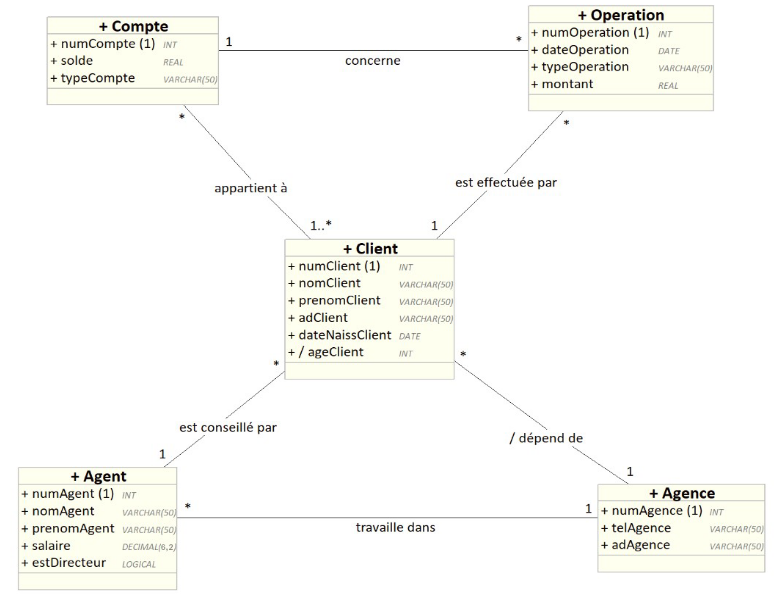
\includegraphics[width=0.9\textwidth]{img/diagramme_bdd.png}
\end{center}

\section{Mise en place de l'environnement}

\subsection{Étape 1 : Configuration Maven}
Ajoutez les dépendances suivantes dans votre fichier \texttt{pom.xml} :

\begin{lstlisting}[language=xml]
<dependencies>
 <!-- JPA API -->
 <dependency>
  <groupId>jakarta.persistence</groupId>
  <artifactId>jakarta.persistence-api</artifactId>
  <version>3.2.0</version>
 </dependency>

 <!-- Implementation JPA (Hibernate) -->
 <dependency>
  <groupId>org.hibernate</groupId>
  <artifactId>hibernate-core</artifactId>
  <version>7.1.11.Final</version>
 </dependency>

 <!-- Base de donnees PostgreSQL -->
 <dependency>
  <groupId>org.postgresql</groupId>
  <artifactId>postgresql</artifactId>
  <version>42.7.8</version>
 </dependency>
</dependencies>
\end{lstlisting}

\subsection{Étape 2 : Configuration JPA}
Créez un fichier \texttt{persistence.xml} dans \texttt{src/main/resources/META-INF/} :

\begin{lstlisting}[language=xml]
<?xml version="1.0" encoding="UTF-8"?>
<persistence version="3.1"
    xmlns="https://jakarta.ee/xml/ns/persistence"
    xmlns:xsi="http://www.w3.org/2001/XMLSchema-instance"
    xsi:schemaLocation="https://jakarta.ee/xml/ns/persistence
    https://jakarta.ee/xml/ns/persistence/persistence_3_1.xsd">

 <persistence-unit name="banquePU" transaction-type="RESOURCE_LOCAL">
  <provider>org.hibernate.jpa.HibernatePersistenceProvider</provider>
  <class>com.votreprojet.model.Client</class>
  <class>com.votreprojet.model.Compte</class>
  <class>com.votreprojet.model.Operation</class>
  <class>com.votreprojet.model.Agent</class>
  <class>com.votreprojet.model.Agence</class>
  
  <properties>
   <property name="jakarta.persistence.jdbc.url"
            value="jdbc:postgresql://localhost:5432/banque_db"/>
   <property name="jakarta.persistence.jdbc.user" value="user"/>
   <property name="jakarta.persistence.jdbc.password" value="password"/>
   <property name="jakarta.persistence.jdbc.driver" value="org.postgresql.Driver"/>
   <property name="hibernate.dialect" value="org.hibernate.dialect.PostgreSQLDialect"/>
   <property name="hibernate.hbm2ddl.auto" value="update"/>
   <property name="hibernate.show_sql" value="true"/>
   <property name="hibernate.format_sql" value="true"/>
  </properties>
 </persistence-unit>
</persistence>
\end{lstlisting}

\section{Entités JPA}

\subsection{Classe Client}
Implémentez la classe \texttt{Client} avec les annotations JPA :

\begin{lstlisting}[language=Java]
package com.votreprojet.model;

import jakarta.persistence.*;
import java.util.Date;
import java.util.List;
@Entity
@Table(name = "Client")
public class Client {
    @Id
    @GeneratedValue(strategy = GenerationType.IDENTITY)
    @Column(name = "numClient")
    private int numClient;

    @Column(name = "nomClient", nullable = false)
    private String nomClient;

    @Column(name = "prenomClient", nullable = false)
    private String prenomClient;

    @Column(name = "adClient")
    private String adClient;

    @Column(name = "dateNaissClient")
    @Temporal(TemporalType.DATE)
    private Date dateNaissClient;

    @Column(name = "ageClient")
    private int ageClient;

    @ManyToOne
    @JoinColumn(name = "numAgent", referencedColumnName = "numAgent")
    private Agent agent;

    @ManyToMany
    @JoinTable(
        name = "Compte_Client",
        joinColumns = @JoinColumn(name = "numClient"),
        inverseJoinColumns = @JoinColumn(name = "numCompte")
    )
    private List<Compte> comptes;

    // Constructeurs, getters et setters
}
\end{lstlisting}

\subsection{Classe Compte}
Implémentez la classe \texttt{Compte} avec les annotations JPA :

\begin{lstlisting}[language=Java]
package com.votreprojet.model;
import jakarta.persistence.*;
import java.util.List;

@Entity
@Table(name = "Compte")
public class Compte {
    @Id
    @GeneratedValue(strategy = GenerationType.IDENTITY)
    @Column(name = "numCompte")
    private int numCompte;

    @Column(name = "solde")
    private double solde;

    @Column(name = "typeCompte", nullable = false)
    private String typeCompte;

    @OneToMany(mappedBy = "compte", cascade = CascadeType.ALL)
    private List<Operation> operations;

    @ManyToMany(mappedBy = "comptes")
    private List<Client> clients;

    // Constructeurs, getters et setters
}
\end{lstlisting}

\section{Patron DAO avec JPA}

\subsection{Interface générique DAO}
Créez une interface générique pour les DAO :

\begin{lstlisting}[language=Java]
package com.votreprojet.dao;

import java.util.List;
import java.util.Optional;

public interface DAO<T, K> {
    Optional<T> find(K id);
    List<T> findAll();
    void save(T entity);
    void update(T entity);
    void delete(T entity);
}
\end{lstlisting}

\subsection{Implémentation générique DAO}
Implémentez une classe générique pour les DAO :

\begin{lstlisting}[language=Java]
package com.votreprojet.dao;

import jakarta.persistence.EntityManager;
import jakarta.persistence.EntityTransaction;
import java.util.List;
import java.util.Optional;

public abstract class AbstractDAO<T, K> implements DAO<T, K> {
    private final Class<T> entityClass;
    protected EntityManager entityManager;

    public AbstractDAO(Class<T> entityClass, EntityManager entityManager) {
        this.entityClass = entityClass;
        this.entityManager = entityManager;
    }

    @Override
    public Optional<T> find(K id) {
        return Optional.ofNullable(entityManager.find(entityClass, id));
    }

    @Override
    public List<T> findAll() {
        return entityManager.createQuery("SELECT e FROM " + entityClass.getSimpleName() + " e", entityClass)
                .getResultList();
    }

    @Override
    public void save(T entity) {
        EntityTransaction transaction = entityManager.getTransaction();
        try {
            transaction.begin();
            entityManager.persist(entity);
            transaction.commit();
        } catch (Exception e) {
            if (transaction != null && transaction.isActive()) {
                transaction.rollback();
            }
            throw e;
        }
    }

    @Override
    public void update(T entity) {
        EntityTransaction transaction = entityManager.getTransaction();
        try {
            transaction.begin();
            entityManager.merge(entity);
            transaction.commit();
        } catch (Exception e) {
            if (transaction != null && transaction.isActive()) {
                transaction.rollback();
            }
            throw e;
        }
    }

    @Override
    public void delete(T entity) {
        EntityTransaction transaction = entityManager.getTransaction();
        try {
            transaction.begin();
            entityManager.remove(entityManager.contains(entity) ? entity : entityManager.merge(entity));
            transaction.commit();
        } catch (Exception e) {
            if (transaction != null && transaction.isActive()) {
                transaction.rollback();
            }
            throw e;
        }
    }
}
\end{lstlisting}

\subsection{DAO Spécifique pour Client}
Créez un DAO spécifique pour la classe \texttt{Client} :

\begin{lstlisting}[language=Java]
package com.votreprojet.dao;

import com.votreprojet.model.Client;
import jakarta.persistence.EntityManager;

public class ClientDAO extends AbstractDAO<Client, Integer> {
    public ClientDAO(EntityManager entityManager) {
        super(Client.class, entityManager);
    }

    public List<Client> findByAgent(int numAgent) {
        return entityManager.createQuery(
            "SELECT c FROM Client c WHERE c.agent.numAgent = :numAgent", Client.class)
            .setParameter("numAgent", numAgent)
            .getResultList();
    }
}
\end{lstlisting}

\section{Patron DTO}

\subsection{DTO pour Client}
Créez une classe DTO pour \texttt{Client} :

\begin{lstlisting}[language=Java]
package com.votreprojet.dto;

import java.util.Date;

public class ClientDTO {
    private int numClient;
    private String nomClient;
    private String prenomClient;
    private String adClient;
    private Date dateNaissClient;
    private int ageClient;
    private int numAgent;

    // Constructeurs, getters et setters
}
\end{lstlisting}

\subsection{Mapper pour Client}
Créez une classe pour mapper les entités aux DTOs :

\begin{lstlisting}[language=Java]
package com.votreprojet.mapper;

import com.votreprojet.dto.ClientDTO;
import com.votreprojet.model.Client;

public class ClientMapper {
    public static ClientDTO toDTO(Client client) {
        ClientDTO dto = new ClientDTO();
        dto.setNumClient(client.getNumClient());
        dto.setNomClient(client.getNomClient());
        dto.setPrenomClient(client.getPrenomClient());
        dto.setAdClient(client.getAdClient());
        dto.setDateNaissClient(client.getDateNaissClient());
        dto.setAgeClient(client.getAgeClient());
        dto.setNumAgent(client.getAgent() != null ? client.getAgent().getNumAgent() : 0);
        return dto;
    }

    public static Client toEntity(ClientDTO dto) {
        Client client = new Client();
        client.setNumClient(dto.getNumClient());
        client.setNomClient(dto.getNomClient());
        client.setPrenomClient(dto.getPrenomClient());
        client.setAdClient(dto.getAdClient());
        client.setDateNaissClient(dto.getDateNaissClient());
        client.setAgeClient(dto.getAgeClient());
        // Note: La relation avec Agent doit etre geree separement
        return client;
    }
}
\end{lstlisting}

\section{Service Layer}

\subsection{Service pour Client}
Créez une classe de service pour gérer la logique métier :

\begin{lstlisting}[language=Java]
package com.votreprojet.service;

import com.votreprojet.dao.ClientDAO;
import com.votreprojet.dto.ClientDTO;
import com.votreprojet.mapper.ClientMapper;
import com.votreprojet.model.Client;
import jakarta.persistence.EntityManager;
import java.util.List;
import java.util.stream.Collectors;

public class ClientService {
    private final ClientDAO clientDAO;

    public ClientService(EntityManager entityManager) {
        this.clientDAO = new ClientDAO(entityManager);
    }

    public ClientDTO createClient(ClientDTO clientDTO) {
        Client client = ClientMapper.toEntity(clientDTO);
        clientDAO.save(client);
        return ClientMapper.toDTO(client);
    }

    public ClientDTO getClient(int id) {
        return clientDAO.find(id)
                .map(ClientMapper::toDTO)
                .orElseThrow(() -> new RuntimeException("Client not found"));
    }

    public List<ClientDTO> getAllClients() {
        return clientDAO.findAll().stream()
                .map(ClientMapper::toDTO)
                .collect(Collectors.toList());
    }

    public List<ClientDTO> getClientsByAgent(int numAgent) {
        return clientDAO.findByAgent(numAgent).stream()
                .map(ClientMapper::toDTO)
                .collect(Collectors.toList());
    }
}
\end{lstlisting}

\section{Application principale}

\subsection{Classe Main}
Créez une classe principale pour tester l'application :

\begin{lstlisting}[language=Java]
package com.votreprojet;

import com.votreprojet.dto.ClientDTO;
import com.votreprojet.service.ClientService;
import jakarta.persistence.EntityManager;
import jakarta.persistence.EntityManagerFactory;
import jakarta.persistence.Persistence;
import java.util.Date;

public class Main {
    public static void main(String[] args) {
        EntityManagerFactory emf = Persistence.createEntityManagerFactory("banquePU");
        EntityManager em = emf.createEntityManager();

        ClientService clientService = new ClientService(em);

        // Exemple de creation d'un client
        ClientDTO clientDTO = new ClientDTO();
        clientDTO.setNomClient("Dupont");
        clientDTO.setPrenomClient("Jean");
        clientDTO.setAdClient("123 Rue de Paris");
        clientDTO.setDateNaissClient(new Date());
        clientDTO.setAgeClient(30);
        clientDTO.setNumAgent(1);

        ClientDTO createdClient = clientService.createClient(clientDTO);
        System.out.println("Client cree: " + createdClient.getNomClient());

        em.close();
        emf.close();
    }
}
\end{lstlisting}

\section{Tâches à réaliser}

\begin{infobox}[P\'erim\`etre du TP (3 s\'eances)]
On se limite aux entit\'es \textbf{Client}, \textbf{Compte} et \textbf{Operation}. Les entit\'es
\texttt{Agent} et \texttt{Agence} sont facultatives.
\end{infobox}

\subsection{Migration de JDBC à JPA}
\begin{enumerate}
\item Migrer les classes métier \texttt{Client}, \texttt{Compte} et \texttt{Operation} en entités JPA (avec leurs relations).
\item Implémenter les DAO de ces trois entités en utilisant la classe générique \texttt{AbstractDAO}.
\item Créer les DTO de \texttt{Client} et \texttt{Compte} et leurs mappers.
\item Implémenter un service \texttt{BanqueService}.
\end{enumerate}

\subsection{Nouvelles fonctionnalités}
\begin{enumerate}
\item Implémenter une méthode pour transférer de l'argent entre deux comptes (avec gestion des transactions).
\item Créer une méthode pour obtenir le solde total d'un client (somme des soldes de tous ses comptes).
\item Implémenter une méthode pour obtenir l'historique des opérations d'un compte.
\end{enumerate}

\subsection{Tests}
\begin{enumerate}
\item Écrire des tests unitaires pour le mapper de \texttt{Client}.
\item Écrire des tests pour la méthode de transfert du service (cas nominal et solde insuffisant).
\end{enumerate}

\subsection{Bonus : observer le problème \og N+1 \fg}
\begin{enumerate}
\item Vérifier que l'affichage des requêtes SQL générées est activé (\texttt{hibernate.show\_sql} et \texttt{hibernate.format\_sql} à \texttt{true} dans \texttt{persistence.xml}, voir plus haut).
\item Charger tous les clients (\texttt{SELECT c FROM Client c}), puis parcourir la liste et afficher le nombre de comptes de chaque client.
      Combien de requêtes SQL sont envoyées pour $N$ clients ?
\item Réécrire la requête avec \texttt{JOIN FETCH} (\texttt{SELECT DISTINCT c FROM Client c LEFT JOIN FETCH c.comptes}) et compter à nouveau.
      Expliquer la différence dans le rapport (lien avec le chapitre 3, Index et optimisation).
\end{enumerate}

\section{Livrables}
\begin{itemize}
\item Un dépôt Git contenant votre code source.
\item Un rapport (fichier Markdown ou PDF) expliquant :
  \begin{itemize}
  \item Les choix techniques que vous avez faits.
  \item Les difficultés rencontrées et comment vous les avez résolues.
  \item Les différences entre l'approche JDBC et JPA.
  \end{itemize}
\item Un fichier Dockerfile et docker-compose.yml mis à jour.
\item Un fichier README.md expliquant comment construire et exécuter votre application.
\end{itemize}

\section{Conseils}
\begin{itemize}
\item Utilisez les transactions pour garantir la cohérence des données.
\item Gérez correctement les exceptions JPA.
\item Utilisez les logs pour tracer les opérations importantes.
\item Testez chaque méthode individuellement avant de passer à la suivante.
\item Respectez les principes SOLID dans votre conception.
\end{itemize}

\end{document}
